\documentclass[a4paper,10pt]{article}

\usepackage[T2A]{fontenc}      
\usepackage[utf8]{inputenc}    
\usepackage[russian]{babel}    

\usepackage{geometry}

\usepackage{graphicx}         

\usepackage{multicol}           

\usepackage{amsmath}           
\usepackage{amssymb}            


\usepackage{array}        


\usepackage{setspace}         


\geometry{margin=0.5cm}
\setstretch{0.9} 

\begin{document}

{\centering
  \small\bfseries КАК УСТРОЕНЫ МЕТАЛЛЫ?\par
}
\vspace{-0.6\baselineskip}

\noindent
\begin{minipage}[t]{0.32\textwidth}
  \raggedright
  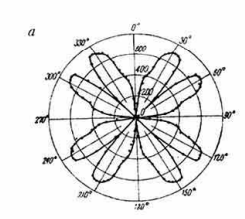
\includegraphics[width=\linewidth]{ris-a}\\[0.5em]
  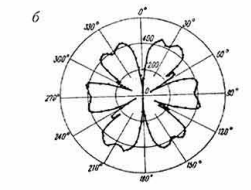
\includegraphics[width=\linewidth]{ris-b}\\[0.5em]
  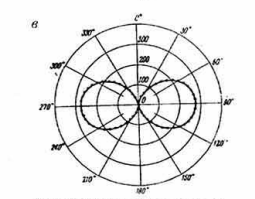
\includegraphics[width=\linewidth]{ris-c}\\[0.5em]

  \small
  \textit{Рис. 3. Изменение сопротивления металла — олова, свинца и таллия
  соответственно при помещении в магнитное поле (в зависимости от
  угла между кристаллическими осями и магнитным полем).}
  \normalsize

  Именно на ней и вокруг этой поверхности находятся электроны,
  играющие важную роль в свойствах металлов.

  \noindent\hrulefill

  \noindent\textbf{Металлы отличаются друг от друга тем, что
  у них разные поверхности Ферми.}

  \noindent\hrulefill

  Прежде чем познакомиться с тем, как узнали, каковы поверхности Ферми
  разных металлов, и какую роль в процессе понимания устройства металлов
  сыграли работы Ильи Михайловича Лифшица и его учеников, посмотрите
  на таблицу. В ней собраны сведения о том, чем похожи и чем отличаются
  электроны в свободном
  
\end{minipage}%
\hfill
\begin{minipage}[t]{0.64\textwidth}

  \begin{multicols}{2}
  \raggedcolumns
  от сил пространстве и в периодическом поле сил
  ионов кристаллической решётки.

  Проблема «устройства» макроскопических, в частности твёрдых, тел
  интересовала И.\,М.~Лифшица с самого начала его научной деятельности.
  Интересы его в большой мере сосредоточивались на решении «обратных»
  задач. Он неоднократно задумывался, нельзя ли по экспериментальным
  данным выяснить, как движутся атомы и электроны в твёрдом теле.
  У него есть небольшая заметка «О колебаниях релятивистских частиц
  в сильных полях». Она опубликована в «Докладах Академии наук СССР»
  в 1948 году (заметки в «Докладах» содержат не более четырёх страниц).
  В заметке выясняется, как по зависимости периода колебаний частицы
  от энергии определить профиль потенциальной ямы, в которой частица
  совершает периодическое движение. Похоже, это — предтеча работ
  с решением «обратных» задач.
  \end{multicols}

  \begin{center}
  {\normalsize
  \renewcommand{\arraystretch}{1.2}
  \setlength{\tabcolsep}{4pt}

  \begin{tabular}{|p{0.48\linewidth}|p{0.48\linewidth}|}
    \hline
    \multicolumn{2}{|c|}{Электрон}\\
    \hline
    \centering в свободном пространстве &
    \centering в кристалле \tabularnewline
    \hline
    \multicolumn{2}{|c|}{состояние характеризуется}\\
    \hline
    \centering импульсом $\vec p$ &
    \centering квазиимпульсом $\vec p$ \tabularnewline
    \hline
    \multicolumn{2}{|c|}{энергия $\varepsilon$}\\
    \hline
    \centering $\displaystyle \varepsilon = \frac{p^{2}}{2m}$ &
    $\varepsilon = \varepsilon(\vec p)$ — периодическая функция
    квазиимпульса \tabularnewline
    \hline
    \multicolumn{2}{|c|}{скорость $\vec v$}\\
    \hline
    \centering $\displaystyle \vec v = \frac{\vec p}{m}$ &
    \centering $\displaystyle \vec v = \frac{d\varepsilon(\vec p)}{d\vec p} \ne \frac{\vec p}{m}$ \tabularnewline
    \hline
    \multicolumn{2}{|c|}{уравнения движения}\\
    \hline
    изменение импульса в ед. времени равно силе $\vec F$ (закон Ньютона):
    \[
      \begin{aligned}
        \frac{\Delta \vec p}{\Delta t} &= \vec F\\[0.3em]
        \frac{\Delta^2 \vec r}{\Delta t^2} &= \frac{\vec F}{m}
      \end{aligned}
    \] &
    изменение квазиимпульса в ед. времени равно внешней силе $\vec F^{\text{вн}}$ (в $\vec F^{\text{вн}}$ не входит периодическая сила ионов):
    {\footnotesize
    \[
      \begin{aligned}
        \frac{\Delta \vec p}{\Delta t} &= \vec F^{\text{вн}}\\[0.3em]
        \frac{\Delta^2 x_i}{\Delta t^2} &= \sum_{k=1}^3 \left(\frac{1}{m^*}\right)_{ik} F^{\text{вн}}_k, \\
        \text{где } & \left(\frac{1}{m^*}\right)_{ik} = \frac{\partial^2\varepsilon(\vec p)}{\partial p_i \partial p_k}
      \end{aligned}
    \]
    }
    \tabularnewline
    \hline
    \multicolumn{2}{|c|}{законы сохранения энергии и импульса (квазиимпульса)}\\
    \hline
    \multicolumn{2}{|c|}{
        \rule{0pt}{1.2em}
        $\varepsilon_1 + \varepsilon_2 = \varepsilon_1' + \varepsilon_2'$
    }\\[0.5em] 
    \centering $\vec p_1 + \vec p_2 = \vec p_1' + \vec p_2'$ &
    \raggedright $\vec p_1 + \vec p_2 = \vec p_1' + \vec p_2' + \vec K$, где $\vec K$ — один из периодов пространства квазиимпульсов \tabularnewline
    \hline
  \end{tabular}
  }
  \end{center}

  \begin{multicols}{2}
  \raggedcolumns
  А в 1954 году Илья Михайлович сформулировал алгоритм, позволяющий
  по тепловым свойствам твёрдых тел получить сравнительно подробную
  характеристику колебательного энергетического спектра твёрдых тел.
  Его метод существенно дополняет широко применяемый метод определения
  колебательного спектра по неупругому рассеянию нейтронов кристаллами.\textsuperscript{4}
  Однако этот метод принципиально не применим для исследования характера
  движения электронов металла. К счастью, в случае электронов есть важное
  облегчающее обстоятельство: нас интересуют не все электроны, а лишь те,
  энергия которых равна энергии Ферми или близка к ней. А это значит, что
  мы должны уметь определять форму поверхности Ферми (см.~(8)) и скорости
  электронов, имеющих фермиевскую энергию. Как обратил внимание Илья
  Михайлович, на помощь приходят свойства кристаллов в магнитном поле
  при низких температурах.

  После первых работ (одну из них я постараюсь схематически изложить)
  возникло направление в исследованиях металлов, ориентированное на
  изучение поверхностей Ферми. Все они построены по такому принципу:
  если поверхность Ферми обладает таким‑то свойством, то наблюдается
  такое‑то явление. По идее, подобные работы должны использоваться
  «в обратном порядке»: наблюдается такое‑то явление — значит, поверхность
  Ферми обладает соответствующим свойством.

  \small
  \noindent\makebox[0.5\linewidth]{\hrulefill}

  \textit{\textsuperscript{4} Пролетая через кристалл, нейтрон может «качнуть»
  атомы кристалла. При этом теряет немного энергии и изменяет направление
  движения. По этим данным определяют, как «качаются» (колеблются) атомы
  кристалла.}

  \normalsize
  \end{multicols}

\end{minipage}

\end{document}